\documentclass[10pt,twocolumn,letterpaper]{article}
\usepackage[left=0.6in,right=0.6in,top=0.7in,bottom=0.7in,columnsep=0.22in,headheight=11pt,headsep=8pt]{geometry}
\usepackage{mathptmx}
\usepackage{amsmath,amssymb}
\usepackage{graphicx}
\usepackage{booktabs}
\usepackage{tabularx}
\usepackage{array}
\usepackage{cite}
\usepackage{fancyhdr}
\usepackage{microtype}
\usepackage[hidelinks]{hyperref}
\usepackage{caption}

\captionsetup{font=footnotesize,labelfont=bf,skip=3pt}
\setlength{\parskip}{0pt}
\setlength{\parindent}{1em}
\setlength{\textfloatsep}{8pt plus 2pt minus 2pt}
\setlength{\dbltextfloatsep}{8pt plus 2pt minus 2pt}
\setlength{\intextsep}{6pt plus 1pt minus 1pt}

\renewcommand{\topfraction}{0.92}
\renewcommand{\dbltopfraction}{0.92}
\renewcommand{\bottomfraction}{0.9}
\renewcommand{\textfraction}{0.07}
\renewcommand{\floatpagefraction}{0.85}
\renewcommand{\dblfloatpagefraction}{0.85}

\pagestyle{fancy}
\fancyhf{}
\fancyhead[L]{\scriptsize NUMA-OTS: NUMA-AWARE TASK SCHEDULING IN OPENMP}
\fancyhead[R]{\scriptsize ABU ZANOUNA AND SEYAM \hspace{0.5em} \thepage}
\renewcommand{\headrulewidth}{0pt}

\makeatletter
\renewcommand{\section}{\@startsection{section}{1}{\z@}%
  {-1.6ex \@plus -0.3ex \@minus -0.2ex}%
  {0.7ex \@plus 0.15ex}%
  {\normalfont\normalsize\centering\scshape}}
\renewcommand{\subsection}{\@startsection{subsection}{2}{\z@}%
  {-1.2ex \@plus -0.25ex \@minus -0.15ex}%
  {0.45ex \@plus 0.1ex}%
  {\normalfont\small\itshape}}
\renewcommand{\thesection}{\Roman{section}}
\renewcommand{\thesubsection}{\Alph{subsection}}
\makeatother

% ---------------------------------------------------------------------------
% Stage 1 Host & Stage 3 Sniper macros (fill in from env_versions.txt,
% host_lscpu.txt, and sniper_cache_energy.csv produced by the pipeline).
\newcommand{\hostcpu}{\textbf{[HOST CPU --- from host\_lscpu.txt]}}
\newcommand{\hostgcc}{\textbf{[GCC VERSION --- from env\_versions.txt]}}
\newcommand{\hostos}{\textbf{[OS / KERNEL --- from env\_versions.txt]}}
% Stage 3 Sniper L3 miss-rate (Base -> OTS) and energy (Base -> OTS) macros:
\newcommand{\sniperSpmvLthree}{\textbf{[SpMV L3\%: Base$\to$OTS from sniper\_cache\_energy.csv]}}
\newcommand{\sniperBfsLthree}{\textbf{[BFS L3\%: Base$\to$OTS from sniper\_cache\_energy.csv]}}
\newcommand{\sniperJoinLthree}{\textbf{[HashJoin L3\%: Base$\to$OTS from sniper\_cache\_energy.csv]}}
\newcommand{\sniperEnergySummary}{\textbf{[Energy mJ: Base$\to$OTS from sniper\_cache\_energy.csv]}}
\newcommand{\TBD}[1]{\textbf{[TBD: #1]}}
% Auto-generated from live simulation CSV outputs by 08_populate_latex_metrics.py
\newcommand{\CaseStudyRows}{%
SpMV & 22.53 & 25.22 & 16.30 & 20.38 & 23.00 & 1.11$\times$ & 26.6\% & 64.83 / 2.34 \\
BFS & 5.09 & 5.13 & 4.46 & 4.93 & 5.75 & 1.03$\times$ & 29.0\% & 52.08 / 2.17 \\
HashJoin & 20.45 & 22.92 & 15.49 & 18.22 & 20.86 & 1.12$\times$ & 26.7\% & 64.88 / 2.34 \\
PageRank & 25.52 & 28.48 & 18.98 & 23.06 & 25.89 & 1.11$\times$ & 26.6\% & 64.95 / 2.34 \\
}

\newcommand{\MainSpeedupRows}{%
SpMV (2N) & 41.53$\pm$0.22 & 40.76 & 44.28 & 42.11 & \textbf{37.24} & 39.09 & 38.51$\pm$0.51 & 1.08$\times$ [1.07,1.08] & 6.4 & $1.12e-08$ & 1.08$\times$ (0.0\%) \\
SpMV (4N) & 22.53$\pm$0.12 & 20.38 & 16.30 & 23.00 & 17.54 & 14.74 & \textbf{14.62$\pm$0.23} & 1.54$\times$ [1.53,1.55] & 26.0 & $1.12e-08$ & 1.67$\times$ (8.2\%) \\
SpMV (8N) & 12.98$\pm$0.11 & 9.95 & 9.39 & 14.39 & \textbf{7.01} & 7.67 & 7.66$\pm$0.02 & 1.69$\times$ [1.69,1.70] & 53.0 & $1.12e-08$ & 1.97$\times$ (16.2\%) \\
\midrule
BFS (2N) & 8.33$\pm$0.08 & 8.44 & 8.78 & 8.58 & \textbf{8.21} & 8.40 & 8.27$\pm$0.03 & 1.01$\times$ [1.00,1.01] & 0.6 & $4.66e-03$ & 1.05$\times$ (4.7\%) \\
BFS (4N) & 5.09$\pm$0.07 & 4.93 & 4.46 & 5.75 & \textbf{4.29} & 4.71 & 4.69$\pm$0.02 & 1.09$\times$ [1.08,1.09] & 5.8 & $1.12e-08$ & 1.29$\times$ (18.9\%) \\
BFS (8N) & 3.60$\pm$0.04 & 3.22 & 3.09 & 4.30 & \textbf{3.08} & 3.62 & 3.59$\pm$0.05 & 1.00$\times$ [1.00,1.01] & 0.2 & $0.159$ (n.s.) & 1.50$\times$ (49.0\%) \\
\midrule
HashJoin (2N) & 37.75$\pm$0.18 & 40.58 & 40.19 & 38.53 & 36.91 & \textbf{36.74} & 37.05$\pm$0.08 & 1.02$\times$ [1.02,1.02] & 4.3 & $1.12e-08$ & 1.03$\times$ (0.7\%) \\
HashJoin (4N) & 20.45$\pm$0.16 & 18.22 & \textbf{15.49} & 20.86 & 16.15 & 15.64 & 15.51$\pm$0.15 & 1.32$\times$ [1.31,1.32] & 24.1 & $1.12e-08$ & 1.46$\times$ (10.9\%) \\
HashJoin (8N) & 11.81$\pm$0.10 & 8.98 & 8.60 & 12.88 & 7.85 & 7.29 & \textbf{7.28$\pm$0.11} & 1.62$\times$ [1.61,1.63] & 38.1 & $1.12e-08$ & 1.85$\times$ (14.1\%) \\
\midrule
PageRank (2N) & 47.32$\pm$0.22 & 49.66 & 50.11 & 47.80 & \textbf{43.95} & 44.69 & 44.10$\pm$0.95 & 1.07$\times$ [1.06,1.08] & 3.1 & $1.12e-08$ & 1.06$\times$ (1.0\%) \\
PageRank (4N) & 25.52$\pm$0.15 & 23.06 & 18.98 & 25.89 & 20.21 & 17.86 & \textbf{17.73$\pm$0.13} & 1.44$\times$ [1.44,1.44] & 47.9 & $1.12e-08$ & 1.57$\times$ (9.0\%) \\
PageRank (8N) & 14.64$\pm$0.12 & 11.35 & 10.73 & 15.98 & \textbf{8.31} & 8.70 & 8.68$\pm$0.05 & 1.69$\times$ [1.68,1.69] & 48.6 & $1.12e-08$ & 1.91$\times$ (13.2\%) \\
}

\newcommand{\AblationRows}{%
\texttt{Base} (central FIFO) & 1.00$\times$ (14.9\%) & 1.00$\times$ (17.5\%) & 1.00$\times$ (14.9\%) & 1.00$\times$ (14.8\%) \\
\texttt{Mem0} (\texttt{--membind=0}) & 0.90$\times$ (15.6\%) & 0.96$\times$ (20.2\%) & 0.90$\times$ (15.6\%) & 0.90$\times$ (15.6\%) \\
\texttt{Inter} (\texttt{--interleave=all}) & 1.38$\times$ (12.4\%) & 1.17$\times$ (13.1\%) & 1.37$\times$ (12.5\%) & 1.36$\times$ (12.4\%) \\
\texttt{ParFT} (static first-touch) & 1.30$\times$ (13.6\%) & 1.12$\times$ (14.5\%) & 1.31$\times$ (16.8\%) & 1.29$\times$ (13.6\%) \\
\texttt{AutoNUMA} (reactive faults) & 0.90$\times$ (16.1\%) & 0.84$\times$ (22.8\%) & 0.92$\times$ (15.8\%) & 0.92$\times$ (16.3\%) \\
M1 only (\texttt{depend} route) & 1.45$\times$ (40.9\%) & 1.14$\times$ (39.7\%) & 1.25$\times$ (40.1\%) & 1.31$\times$ (40.0\%) \\
M2 only (gated migration) & 0.94$\times$ (16.0\%) & 0.88$\times$ (22.7\%) & 0.95$\times$ (15.6\%) & 0.95$\times$ (16.0\%) \\
M3 only (3-tier SLIT queues) & 1.00$\times$ (14.9\%) & 0.98$\times$ (14.1\%) & 1.01$\times$ (16.1\%) & 1.00$\times$ (14.9\%) \\
M1 + M2 (no SLIT queues) & 1.28$\times$ (49.3\%) & 0.96$\times$ (40.7\%) & 1.25$\times$ (46.6\%) & 1.27$\times$ (48.9\%) \\
M1 + M3 (no migration) & 1.85$\times$ (72.7\%) & 1.17$\times$ (64.8\%) & 1.50$\times$ (72.7\%) & 1.76$\times$ (72.6\%) \\
M2 + M3 (no \texttt{depend} M1) & 0.91$\times$ (12.7\%) & 0.84$\times$ (14.1\%) & 0.93$\times$ (14.8\%) & 0.92$\times$ (12.6\%) \\
Ungated M2 ($\gamma{=}1.0, T_{\mathrm{cool}}{=}0$) & 1.69$\times$ (82.9\%) & 1.00$\times$ (66.4\%) & 1.62$\times$ (79.9\%) & 1.68$\times$ (82.8\%) \\
\textbf{Full NUMA-OTS (M1+M2+M3)} & \textbf{1.69$\times$ (82.9\%)} & \textbf{1.00$\times$ (66.4\%)} & \textbf{1.62$\times$ (80.0\%)} & \textbf{1.69$\times$ (82.9\%)} \\
}

\newcommand{\TelemetryEightNodeRows}{%
\texttt{Base} $\alpha_{\mathrm{loc}}$ & 14.9\% & 17.5\% & 14.9\% & 14.8\% \\
\textbf{Full OTS $\alpha_{\mathrm{loc}}$} & \textbf{82.9\%} & \textbf{66.4\%} & \textbf{80.0\%} & \textbf{82.9\%} \\
\texttt{Base} $T_{\mathrm{cont}}$ (ns) & 60.45 & 48.55 & 60.18 & 60.31 \\
\textbf{Full OTS $T_{\mathrm{cont}}$ (ns)} & \textbf{6.19} & \textbf{17.74} & \textbf{11.73} & \textbf{7.76} \\
Memory-stall fraction $f_{\mathrm{mem}}$ & 0.878 & 0.834 & 0.898 & 0.843 \\
Migrations / trial (Ungated $\to$ Full) & 472.5$\to$465.3 & 176.1$\to$156.9 & 384.0$\to$384.0 & 473.6$\to$468.3 \\
\textbf{6-Epoch re-migs (Ungated $\to$ Full)} & \textbf{8.9$\to$6.4} & \textbf{10.0$\to$0.0} & \textbf{5.4$\to$5.0} & \textbf{8.5$\to$6.0} \\
\textbf{Beneficial migration precision (Full)} & \textbf{96.4\%} & \textbf{83.8\%} & \textbf{96.0\%} & \textbf{96.5\%} \\
Critical-path mig.\ pause (ms, Full) & 1.417 & 0.599 & 1.114 & 1.418 \\
Total overhead (\% of makespan, Full) & 19.01\% & 16.88\% & 15.79\% & 16.84\% \\
Stage~1 DES LLC miss (\% Base $\to$ Full) & 43.6$\to$29.4 & 44.0$\to$42.3 & 43.0$\to$30.8 & 43.6$\to$29.5 \\
Dynamic energy (mJ, Base $\to$ Full) & 176.0$\to$114.7 & 35.6$\to$27.7 & 158.1$\to$104.9 & 202.5$\to$134.4 \\
Total energy (mJ, Base $\to$ Full) & 2044.6$\to$1218.0 & 554.4$\to$544.7 & 1858.3$\to$1152.4 & 2310.1$\to$1383.6 \\
}

\newcommand{\ControllerAccountingRows}{%
SpMV & 1024 & 1932 & 1300$\to$244 & 180 & 251.6k$\to$86.8k & 0.88$\to$0.48 & 88.0$\to$12.9 \\
BFS & 129 & 1542 & 1040$\to$418 & 280 & 99.2k$\to$48.0k & 0.34$\to$0.27 & 23.9$\to$15.7 \\
HashJoin & 768 & 1932 & 1293$\to$304 & 220 & 305.5k$\to$116.5k & 0.88$\to$0.65 & 88.0$\to$28.8 \\
PageRank & 1024 & 1932 & 1298$\to$242 & 200 & 278.6k$\to$96.4k & 0.88$\to$0.54 & 88.0$\to$17.0 \\
}

\newcommand{\SpdRangeAll}{$1.00\times$ to $1.69\times$}
\newcommand{\SpdRangeIterTwo}{$1.02\times$--$1.08\times$}
\newcommand{\SpdRangeIterFour}{$1.32\times$--$1.54\times$}
\newcommand{\SpdRangeIterEight}{$1.62\times$--$1.69\times$}
\newcommand{\MaxPHolmSig}{$p_{\mathrm{Holm}} \le 4.66e-03$}
\newcommand{\AlphaBaseEightRange}{$14.8\%$--$17.5\%$}
\newcommand{\AlphaOtsEightIterRange}{$80.0\%$--$82.9\%$}
\newcommand{\AlphaOtsEightAllRange}{$66.4\%$--$82.9\%$}
\newcommand{\AlphaOtsEightBfs}{$66.4\%$}
\newcommand{\TcontRedRange}{$63.5\%$--$89.8\%$}
\newcommand{\TcontBaseEightRange}{$48.55$--$60.45$\,ns}
\newcommand{\TcontOtsEightRange}{$6.19$--$17.74$\,ns}
\newcommand{\OvhdRangeAll}{$0.38\%$--$19.01\%$}
\newcommand{\OvhdRangeEight}{$15.79\%$--$19.01\%$}
\newcommand{\DynEnergyRedRange}{$22.0\%$--$34.8\%$}
\newcommand{\TotEnergyRedRange}{$1.7\%$--$40.4\%$}
\newcommand{\TotEnergyRedIterRange}{$38.0\%$--$40.4\%$}
\newcommand{\TotEnergyRedBfs}{$1.7\%$}
\newcommand{\DesLlcBaseRange}{$43.0\%$--$44.0\%$}
\newcommand{\DesLlcOtsRange}{$29.4\%$--$42.3\%$}
\newcommand{\CaseStudyAlphaRange}{$26.6\%$--$29.0\%$}
\newcommand{\CaseStudyTcontRange}{$52.08$--$64.95$\,ns}
\newcommand{\CaseStudyGammaRange}{$2.17$--$2.34$}
\newcommand{\CaseStudyBaseParftRange}{$1.03\times$--$1.12\times$}
\newcommand{\SpmvSpdAll}{$1.08\times$ (2N), $1.54\times$ (4N), and $1.69\times$ (8N)}
\newcommand{\PrSpdAll}{$1.07\times$ (2N), $1.44\times$ (4N), and $1.69\times$ (8N)}
\newcommand{\JoinSpdAll}{$1.02\times$ (2N), $1.32\times$ (4N), and $1.62\times$ (8N)}
\newcommand{\JoinInterFullRange}{$1.00\times$--$1.18\times$}
\newcommand{\BfsSpdAll}{$1.01\times$ (2N), $1.09\times$ (4N), and $1.00\times$ (8N)}
\newcommand{\BfsMthirteenAll}{$1.01\times$ (2N), $1.19\times$ (4N), and $1.17\times$ (8N)}
\newcommand{\BfsRfPredEight}{$1.50\times$}
\newcommand{\BfsRfErrEight}{$49.0\%$}
\newcommand{\IterRfErrRange}{$0.0\%$--$16.2\%$}
\newcommand{\MemZeroBeatRange}{$1.04\times$--$1.89\times$}
\newcommand{\InterBeatRange}{$0.86\times$--$1.24\times$}
\newcommand{\ParFtBeatRange}{$0.90\times$--$1.39\times$}
\newcommand{\AutoNumaBeatRange}{$1.04\times$--$1.88\times$}
\newcommand{\ReSixSummary}{SpMV $8.9 \to 6.4$, BFS $10.0 \to 0.0$, HashJoin $5.4 \to 5.0$, and PageRank $8.5 \to 6.0$ (beneficial migration precision $83.8\%$--$96.5\%$)}
\newcommand{\EpycEightSummary}{$1.72\times$ on SpMV, $0.98\times$ on BFS, $1.64\times$ on HashJoin, $1.71\times$ on PageRank}
\newcommand{\HookSummaryText}{intercepted $2,950$ \texttt{GOMP\_task} calls ($2,948$ with \texttt{depend} clauses, i.e., $99.93\%$), parsed $5,764$ locators with an $82.8\%$ PHHT hit ratio ($4,772$ hits, $992$ misses across $909$ per-task \texttt{move\_pages(2)} query syscalls; mean query batch $1.09$ pages/call), and submitted $216$ M2 page-migration requests across $9$ non-empty batches out of $27$ \texttt{GOMP\_taskwait} epochs (mean request batch $B=24.00$, max $49$ pages; $0$ kernel-confirmed cross-node moves on the single-node WSL2 host)}
\newcommand{\BatchHistSummary}{mean DES migration batch sizes on 8~domains are SpMV: $58.2$ (max 64), BFS: $39.2$ (max 64), HashJoin: $64.0$ (max 64), PageRank: $58.8$ (max 64)}
\newcommand{\GranSweepSummary}{8N BFS Full NUMA-OTS scales from $0.94\times$ at $19\,\mu$s to $1.01\times$ at $320\,\mu$s and $1.18\times$ at $2560\,\mu$s (vs.\ \texttt{M1+M3} at $1.17\times$), while 8N SpMV scales from $1.83\times$ to $2.02\times$}
\newcommand{\SensSweepSummary}{sweeping $\gamma \in [0.5, 3.0]$ on 8N SpMV yields $1.70\times$ at $\gamma=1.5$ vs.\ $1.71\times$ at $\gamma=3.0$; sweeping $T_{\mathrm{rem}}/T_{\mathrm{loc}} \in [1.25, 3.00]$ on 4N SpMV increases speedup monotonically from $1.35\times$ to $1.92\times$; sweeping misses/page/sweep $\in [2, 100]$ ($\times 10$ sweeps/phase) on 8N SpMV rises from $1.03\times$ at $2$ to a peak of $1.71\times$ at $20$ before all-controller saturation compresses speedup to $1.21\times$ at $100$; sweeping $f_{\mathrm{mem}} \in [0.21, 0.95]$ scales 8N SpMV speedup from $1.23\times$ to $1.72\times$; varying initial Node-0 page skew from $0\%$ to $100\%$ shifts 8N SpMV speedup from $1.31\times$ to $1.75\times$}

% ---------------------------------------------------------------------------

\begin{document}

\twocolumn[{%
\begin{center}
{\LARGE\bfseries NUMA-Aware Task Scheduling for Shared-Memory Parallel Applications Using OpenMP\par}
\vspace{0.5em}
{\large Khalil Ibrahim Abu Zanouna$^1$ and Mohammed Abdulsalam Seyam$^2$\par}
\vspace{0.2em}
{\small\itshape $^{1,2}$Computer Engineering Department, Faculty of Engineering, Islamic University of Gaza, Gaza, Palestine\par}
{\small\itshape E-mail: khalil500863335@gmail.com, moh.seyam0@gmail.com\par}
\vspace{0.6em}
\end{center}
\noindent{\small\textbf{\textit{Abstract}---Multi-socket servers partition physical memory into non-uniform memory access (NUMA) domains, yet mainstream OpenMP runtimes schedule explicit tasks without tracking where their data reside, inflating remote DRAM latency and memory-controller queueing. We present NUMA-OTS, a NUMA-aware OpenMP task scheduler and drop-in \texttt{LD\_PRELOAD} runtime extension for GNU \texttt{libgomp} that combines (M1) first-touch-aware task placement guided by \texttt{depend}-clause locators and a user-space Page-Home Hash Table (PHHT), (M2) access-frequency-guided page migration gated by a multi-domain cost-benefit model with hysteresis, cooldown, and a controller-congestion guard, and (M3) hierarchical core-, domain-, and team-level task queues with topology-ordered work stealing. We evaluate NUMA-OTS through a reproducible three-level methodology: (Stage~1) live OpenMP task trace extraction across sparse matrix-vector multiplication (SpMV), breadth-first search (BFS), morsel-driven hash join, and iterative PageRank feeding a pure-C11 discrete-event simulator of 2-, 4-, and 8-domain Intel Xeon and AMD EPYC topologies over 30 paired trials; (Stage~2) functional OS/syscall verification of \texttt{libnuma}, \texttt{hwloc}, \texttt{move\_pages(2)}, and \texttt{LD\_PRELOAD} \texttt{GOMP\_task} interposition inside a 4-node virtual NUMA Linux guest under QEMU; and (Stage~3) instruction- and cycle-level L1/L2/L3 cache-miss and energy characterization via Valgrind Cachegrind and Sniper/McPAT. Across all four benchmarks, we quantify simulated speedups (\TBD{speedup range from summary\_table.csv}), remote DRAM access reduction, controller queueing relief, cache-miss and energy savings, and the task-granularity and phase-length thresholds governing dynamic page migration.}\par}
\vspace{0.3em}
\noindent{\small\textbf{\textit{Index Terms}---Data locality, discrete-event simulation, memory hierarchy, non-uniform memory access (NUMA), OpenMP, task scheduling, work stealing.}\par}
\vspace{0.7em}
}]

% ===========================================================================
\section{Introduction}

\subsection{NUMA Ubiquity in Modern Servers}
Contemporary multi-socket server processors partition physical memory across distributed locality domains to overcome the bus saturation of centralized shared-memory architectures \cite{ref1,ref2}. Within each NUMA domain, processor cores connect directly to integrated DRAM controllers, scaling aggregate memory bandwidth with socket count \cite{ref3,ref4}. When a core accesses cache lines hosted on a remote domain, coherence transactions traverse inter-socket point-to-point interconnects. Uncoordinated thread scheduling and page placement amplify remote link traffic and memory-controller queueing delays, reducing performance by 30--60\% in reported memory-intensive NUMA workloads \cite{ref5,ref6}. Because even single-socket parts now expose several NUMA domains under Sub-NUMA Clustering (SNC) or NUMA-per-Socket (NPS) modes \cite{ref21}, locality-aware scheduling is a mainstream rather than a niche concern.

\subsection{OpenMP's Locality Gap}
OpenMP 5.2 provides portable directives for explicit tasking (\texttt{task}, \texttt{taskloop}), sibling data-flow ordering (\texttt{depend}), and thread pinning (\texttt{OMP\_PLACES}, \texttt{OMP\_PROC\_BIND}), but leaves page-residency-aware task scheduling unspecified \cite{ref7}. In GNU \texttt{libgomp} (GCC 13.2.0), ready-task insertion uses dependence tokens solely for execution ordering without querying which NUMA domain hosts the referenced physical frames \cite{ref8}. While dynamic work stealing balances irregular task trees \cite{ref9}, unguided cross-socket steals separate computation from its data and inflate remote interconnect traffic \cite{ref10,ref11}.

Prior runtimes address distinct facets of this problem, including hierarchical thread-team bubbles in ForestGOMP \cite{ref12}, explicit region-footprint extensions in MIR \cite{ref13}, chip-level shared queues \cite{ref10}, and streaming data-flow compilers \cite{ref11}; Section~II contrasts these designs. We study how dependence-locator-guided placement, sampled page migration, and topology-aligned queues interact under \emph{standard} OpenMP tasking semantics, guided by two research questions:
\begin{itemize}\setlength{\itemsep}{0pt}\setlength{\parskip}{0pt}\setlength{\topsep}{2pt}
\item \textit{RQ1}: Across what ranges of per-task duration ($\tau_{\mathrm{task}}$) and domain counts ($N_{\mathrm{dom}} \in \{2, 4, 8\}$) does combining residency-guided task routing with topology-aligned queues reduce remote DRAM accesses and execution time relative to a NUMA-oblivious baseline?
\item \textit{RQ2}: Under what phase-length, hysteresis ($\gamma$), cooldown ($T_{\mathrm{cool}}$), and controller-utilization thresholds does dynamic page migration yield net latency savings exceeding its transfer and TLB-shootdown overheads, and when is it better to disable migration?
\end{itemize}

\subsection{Contributions: Design, Implementation, Evaluation}
To remain reproducible and to avoid claiming unmeasured bare-metal results, this work makes three contributions:
\begin{itemize}\setlength{\itemsep}{1pt}\setlength{\parskip}{0pt}\setlength{\topsep}{2pt}
\item \textbf{Design.} The NUMA-OTS architecture (Fig.~\ref{fig:arch}, Sec.~IV): (M1) read-only \texttt{depend}-locator residency scoring backed by a Page-Home Hash Table (PHHT); (M2) multi-domain cost-benefit-gated page migration with a stabilized EMA demand predictor, hysteresis, cooldown, and a controller-congestion guard; (M3) per-team three-tier topology-aligned queues with SLIT-ordered work stealing; and a binary-compatible \texttt{LD\_PRELOAD} runtime interposition design for \texttt{libgomp}.
\item \textbf{Implementation.} An open, multi-level runtime and simulation suite (Sec.~V): an \texttt{LD\_PRELOAD} shared library (\texttt{libnuma\_ots\_hook.so}) intercepting \texttt{GOMP\_task} and \texttt{GOMP\_taskwait}; an automated unit and concurrency stress-test suite; an OpenMP trace extractor feeding a pure-C11 min-heap discrete-event simulator (DES) of Intel Xeon and AMD EPYC topologies with explicit \texttt{depend} readiness, phase barriers, three-tier queues, M/M/1 controller queueing, LLC residency, and RAPL/McPAT energy accounting; a 4-node QEMU virtual-NUMA verifier; and micro-kernels for Valgrind Cachegrind and Sniper.
\item \textbf{Evaluation.} Paired simulation experiments across 7 policies, 4 workloads (SpMV, BFS, HashJoin, PageRank), and 2, 4, and 8 NUMA domains (30 paired trials per configuration) plus a 240-run task-granularity sweep (Sec.~VI), reporting 95\% paired bootstrap confidence intervals, Holm--Bonferroni-adjusted Wilcoxon tests, effect sizes ($d_z$), comparisons against \texttt{numactl}-equivalent policies, and both positive and negative regimes.
\end{itemize}
Section~II reviews background and related work, Section~III quantifies the problem, Sections~IV and V present the design and its implementation, Section~VI evaluates it, Section~VII discusses trade-offs and limitations, and Section~VIII concludes.

% ===========================================================================
\section{Background}

\subsection{NUMA Architecture Fundamentals}
Classical uniform-memory-access (UMA) multiprocessors route memory requests over a shared bus or crossbar \cite{ref20}. As core counts scale, centralized controllers saturate; ccNUMA servers therefore distribute physical memory across $N_{\mathrm{dom}}$ locality domains, configured either as one domain per socket or as several intra-socket domains under SNC/NPS \cite{ref21}. Cache-sharing boundaries (L2/LLC slices) need not map one-to-one onto NUMA boundaries \cite{ref22}.

Under a first-order mean-value approximation with effective memory-level parallelism (MLP), the expected service latency of an LLC miss that reaches DRAM is
\begin{equation}
E[T_{\mathrm{mem}} \mid \text{DRAM miss}] = \alpha_{\mathrm{loc}}\, T_{\mathrm{loc}} + (1 - \alpha_{\mathrm{loc}})\,\overline{T}_{\mathrm{rem}} + T_{\mathrm{cont}}(\lambda),
\label{eq:latency}
\end{equation}
where $\alpha_{\mathrm{loc}} \in [0,1]$ is the local DRAM hit fraction, $T_{\mathrm{loc}}$ the unloaded local latency, $\overline{T}_{\mathrm{rem}} > T_{\mathrm{loc}}$ the distance-weighted unloaded remote latency, and $T_{\mathrm{cont}}(\lambda) \ge 0$ the controller queueing delay under request-rate vector $\lambda$. Because ACPI SLIT tables (Sec.~5.2.17 of \cite{ref23}) report normalized relative distances rather than nanoseconds, latency matrices $L(w,x)$ must be calibrated from pointer-chasing measurements; prior studies \cite{ref24} emphasize that $T_{\mathrm{cont}}(\lambda)$ can dominate stall time when hot pages saturate one controller.

Under the Roofline model \cite{ref25}, for a memory-bound kernel whose DRAM stalls form a fraction $f_{\mathrm{mem}} \in (0,1]$ of its ideal all-local runtime, relative runtime scales with the latency inflation factor $\Gamma = E[T_{\mathrm{mem}}]/T_{\mathrm{loc}}$ as
\begin{equation}
T_{\mathrm{rel}} \approx (1 - f_{\mathrm{mem}}) + f_{\mathrm{mem}}\,\Gamma .
\label{eq:roofline}
\end{equation}
We use Eqs.~(\ref{eq:latency})--(\ref{eq:roofline}) to quantify the problem (Sec.~III) and to cross-check the simulator (Sec.~VI-D).

\subsection{OpenMP Tasking Model (\texttt{task}, \texttt{taskloop}, \texttt{depend})}
An OpenMP \texttt{task} packages a code block and its data environment for deferred execution by any thread of the binding team; \texttt{taskwait}, \texttt{taskgroup}, and barriers provide completion synchronization. \texttt{taskloop} partitions a loop into tasks by \texttt{grainsize} or \texttt{num\_tasks}. The \texttt{depend} clause (\texttt{in}, \texttt{out}, \texttt{inout}, \texttt{mutexinoutset}, \texttt{inoutset}) orders sibling tasks by the storage locations they name. OpenMP 5.2 specifies tasking in Secs.~12.5--12.6, task scheduling constraints (TSCs) in Sec.~12.9, dependences in Sec.~15.9.5, and affinity in Secs.~21.1.6--21.1.7 \cite{ref7}. OpenMP 5.2 does \emph{not} permit \texttt{depend} on \texttt{taskloop} (deferred to OpenMP 6.0 \texttt{task\_iteration}), and the OpenMP 5.0 \texttt{affinity} clause is accepted but ignored by GCC 13.2.0.

In GCC 13.2.0 \texttt{libgomp} (\texttt{libgomp.h}, \texttt{task.c}) \cite{ref8}, tasks traverse team-level (\texttt{team->task\_queue}, with priority subqueues under \texttt{team->task\_lock}), parent-level (\texttt{children\_queue}, \texttt{depend\_hash}), and \texttt{taskgroup\_queue} scopes. When GCC emits \texttt{GOMP\_task} for array sections (\texttt{a[0:N]}), the ABI passes only base addresses, not byte extents \cite{ref16}. NUMA-OTS therefore treats \texttt{depend} locators strictly as approximate base-page locality hints.

\subsection{Existing NUMA-Aware Tools: numactl, LIKWID, hwloc}
\texttt{numactl}/\texttt{libnuma} \cite{ref14} applies process-wide memory policies (e.g., \texttt{--membind}, \texttt{--interleave}) and exposes \texttt{move\_pages(2)}; it is static and task-blind. LIKWID \cite{ref26} pins threads and reads hardware performance counters but does not place tasks or pages. \texttt{hwloc} \cite{ref22} discovers the topology (SLIT distances, caches, cores) and offers binding APIs, serving as a substrate on which runtimes such as NUMA-OTS would build. We emulate the two most common \texttt{numactl} policies as baselines in Sec.~VI.

\subsection{Related Work in Thread and Data Placement}
Table~\ref{tab:comparison} positions NUMA-OTS against OS kernel policies (Carrefour \cite{ref6}, kMAF \cite{ref27}, Linux AutoNUMA \cite{ref21}) and task/data-flow runtimes (ForestGOMP \cite{ref12}, Olivier et al. \cite{ref10}, OpenStream \cite{ref11}, MIR \cite{ref13}, StarPU, OmpSs-2/Nanos6, and Qthreads). Kernel policies react to minor page faults or PMU samples at OS-thread granularity without visibility into user-space OpenMP task DAGs. Alternative tasking runtimes such as StarPU, OmpSs-2/Nanos6, and Qthreads provide locality-aware work descriptors and shepherd queues, and OpenMP 5.0 introduced an \texttt{affinity} clause for task-data locality hints \cite{ref7}; however, \texttt{affinity} remains a no-op stub in GCC 13.2.0 \texttt{libgomp} \cite{ref8}, while custom runtimes require either non-standard compiler extensions \cite{ref11,ref13} or omit dynamic page migration \cite{ref10,ref13}. NUMA-OTS derives locality directly from standard OpenMP \texttt{depend} clauses via binary-compatible \texttt{LD\_PRELOAD} interposition and couples task placement with cost-benefit-gated page migration.

\begin{table*}[!t]
\centering
\caption{Comparison of System-Level NUMA Utilities, OS/Runtime Placement Policies, and the Proposed NUMA-OTS Design}
\label{tab:comparison}
\resizebox{\textwidth}{!}{%
\begin{tabular}{@{}l p{2.4cm} p{2.7cm} p{3.0cm} p{3.6cm} p{3.1cm}@{}}
\toprule
\textbf{System / Tool} & \textbf{Control Scope} & \textbf{Locality Signal} & \textbf{Queue \& Steal Design} & \textbf{Page Migration Policy} & \textbf{OpenMP Binary Compatibility} \\
\midrule
\texttt{numactl} / \texttt{libnuma} \cite{ref14} & OS process / VMA & Static CLI flags (\texttt{membind}, \texttt{interleave}) & None (OS scheduler / baseline OpenMP) & Manual syscall API (\texttt{move\_pages}); no task policy & External CLI/library wrapper (task-blind) \\
LIKWID (\texttt{likwid-pin}) \cite{ref26} & POSIX / OpenMP threads & Core/socket topology IDs + PMU counters & None (pins threads via \texttt{LD\_PRELOAD}) & None (thread pinning and PMU profiling) & External wrapper (task-blind) \\
\texttt{hwloc} \cite{ref22} & Topology tree / bitmaps & ACPI SLIT, \texttt{sysfs}, \& cache hierarchy & None (substrate library for runtimes) & Explicit binding API ({\small\texttt{HWLOC\_MEMBIND\_MIGRATE}}) & Library API (requires runtime integration) \\
Carrefour \cite{ref6} & OS kernel threads \& pages & Hardware PMU instruction sampling & OS thread clustering (no task-DAG visibility) & Reactive kernel replication, interleaving, \& migration & Kernel patch (no user task-DAG API) \\
kMAF \cite{ref27} & OS kernel threads \& pages & Minor page faults \& TLB miss tracking & OS affinity grouping (no task-DAG visibility) & Reactive kernel thread \& page co-migration & Kernel patch (no user task-DAG API) \\
ForestGOMP \cite{ref12} & Nested \texttt{omp parallel} teams & Thread-team bubble tree over \texttt{hwloc} & Hierarchical Marcel bubble stealing & Explicit \& next-touch migration via MAMI & Modified \texttt{libgomp} + Marcel/MAMI stack \\
Olivier et al. \cite{ref10} & Unstructured \texttt{omp task} & Chip-level shared LLC topology & Shared per-chip LIFO + designated thief & Dynamic page migration not evaluated & Custom tasking runtime prototype \\
OpenStream \cite{ref11} & Data-flow streaming tasks & Compiler-emitted stream frame descriptors & Per-worker deques with locality push & Adaptive data-frame placement at runtime & No (requires OpenStream compiler) \\
Muddukrishna et al. \cite{ref13} & Dependent OpenMP tasks & Explicit region byte extents / \texttt{depend} (MIR) & Per-node queues; footprint \& distance routing & Static initial distribution; no dynamic migration & Extended OpenMP / custom MIR runtime \\
\textbf{NUMA-OTS (This Work)} & \textbf{Standard \texttt{omp task} (modeled runtime)} & \textbf{\texttt{depend} base pages + PHHT \& modeled PMU} & \textbf{Per-team topology-aligned 3-tier queues} & \textbf{Multi-domain net-gain, cooldown, \& congestion-gated migration} & \textbf{Designed for GCC 13.2.0 ABI; evaluated via C11 DES} \\
\bottomrule
\end{tabular}%
}
\end{table*}

% ===========================================================================
\section{Motivation and Problem Analysis}

\subsection{Quantifying the Remote Memory Penalty}
With the calibrated latencies used throughout this paper ($T_{\mathrm{loc}}=84$\,ns, 149\,ns at one hop, 186\,ns at two hops; Sec.~VI-A), a remote access costs $1.77\times$ a local one at one hop and $2.21\times$ at two hops; on the 8-domain topology the distance-weighted mean remote latency ($\overline{T}_{\mathrm{rem}}=170.1$\,ns) is $2.03\times$ $T_{\mathrm{loc}}$. A NUMA-oblivious schedule leaves only about $1/N_{\mathrm{dom}}$ of accesses local, so even without contention Eq.~(\ref{eq:latency}) gives $\Gamma = 1.39$, $1.58$, and $1.90$ for 2, 4, and 8 domains. For a memory-bound kernel with $f_{\mathrm{mem}} = 0.88$ (typical of our traces, Table~\ref{tab:telemetry}), Eq.~(\ref{eq:roofline}) predicts slowdowns of $1.34\times$, $1.51\times$, and $1.79\times$ relative to an all-local execution, before any queueing. Controller contention adds a further 16--40\,ns per miss under the baseline across our nine simulated configurations ($0.19$--$0.48\,T_{\mathrm{loc}}$), so the penalty grows with domain count exactly where multi-socket servers are meant to scale.

\subsection{Case Study: Default OpenMP on a Simulated 4-Socket System}
Table~\ref{tab:casestudy} isolates the simulated 4-socket configuration across the four workloads. The NUMA-oblivious baseline (central task queue over mixed first-touch pages, Sec.~VI-D) leaves most DRAM misses remote (\TBD{4N baseline $\alpha_{\mathrm{loc}}$ from Table III}) and incurs significant controller queueing delay per miss (\TBD{4N baseline $T_{\mathrm{cont}}$ and $\Gamma$ from Table III}), running \TBD{4N Base/ParFT slowdown range} slower than the ideal static \texttt{ParFT} reference. Process-wide \texttt{numactl} policies do not close this gap: binding all memory to Node~0 (\texttt{Mem0}) exacerbates controller contention because a single memory controller absorbs all traffic, while round-robin interleaving (\texttt{Inter}) balances controllers without improving task-to-page locality.

\begin{table}[!t]
\centering
\caption{Simulated 4-Socket Case Study (Mean of 30 Trials): Execution Time (ms) of the Default NUMA-Oblivious Schedule, \texttt{numactl}-Equivalent Policies, and Ideal Static Placement, with Baseline Locality and Queueing Telemetry}
\label{tab:casestudy}
\resizebox{\columnwidth}{!}{%
\begin{tabular}{@{}lccccccc@{}}
\toprule
\textbf{Workload} & \textbf{Base} & \textbf{Mem0} & \textbf{Inter} & \textbf{ParFT} & \textbf{Base/ParFT} & $\boldsymbol{\alpha_{\mathrm{loc}}}$ & $\boldsymbol{T_{\mathrm{cont}}}$ \textbf{(ns)} / $\boldsymbol{\Gamma}$ \\
\midrule
\CaseStudyRows
\bottomrule
\end{tabular}%
}
\end{table}

\subsection{Sources of Imbalance: Page Placement, Task Stealing, Cache Effects}
\textit{Page placement.} Linux allocates a page on the domain of the thread that first touches it \cite{ref21}. Initialization loops and dynamically created tasks rarely agree, and hot shared structures---the SpMV source vector $x$, the BFS \texttt{dist} array, and the hash-join build table---concentrate on whichever domain touched them first. Our simulator models this mixed first-touch state by homing 60\% of the pages of these three structures on Node~0 and block-distributing all other arrays.

\textit{Task stealing.} A central queue (or unguided stealing) hands the next ready task to whichever worker becomes idle, so the probability that the executing worker shares a domain with the task's data is roughly $1/N_{\mathrm{dom}}$. Lock contention on the shared queue also grows with domain count (modeled as $110 + 18N_{\mathrm{dom}}$\,ns per dispatch).

\textit{Cache effects.} Cross-domain execution also forfeits warm LLC contents and generates coherence traffic. Our simulator does not model caches explicitly; their effect is folded into the constant MLP factor (Sec.~VII-C). NUMA-OTS addresses the first two sources directly: M1 and M3 move tasks to data, and M2 moves persistently remote data to its consumers.

% ===========================================================================
\section{NUMA-OTS Design}

\subsection{Architecture Overview}
Figure~\ref{fig:arch} shows the NUMA-OTS architecture together with the simulation pipeline used to evaluate it, and Table~\ref{tab:symbols} summarizes the notation. When a task is created, M1 scores the NUMA domains that host its \texttt{depend} locators and routes the task to one of M3's three queue tiers. Idle workers search the tiers in locality-first order. At each epoch boundary (a barrier or phase end), M2 consumes sampled per-page demand and migrates pages whose projected gain exceeds a hysteresis-scaled cost, updating the PHHT so that subsequent placements follow the data.

\begin{figure*}[!t]
\centering
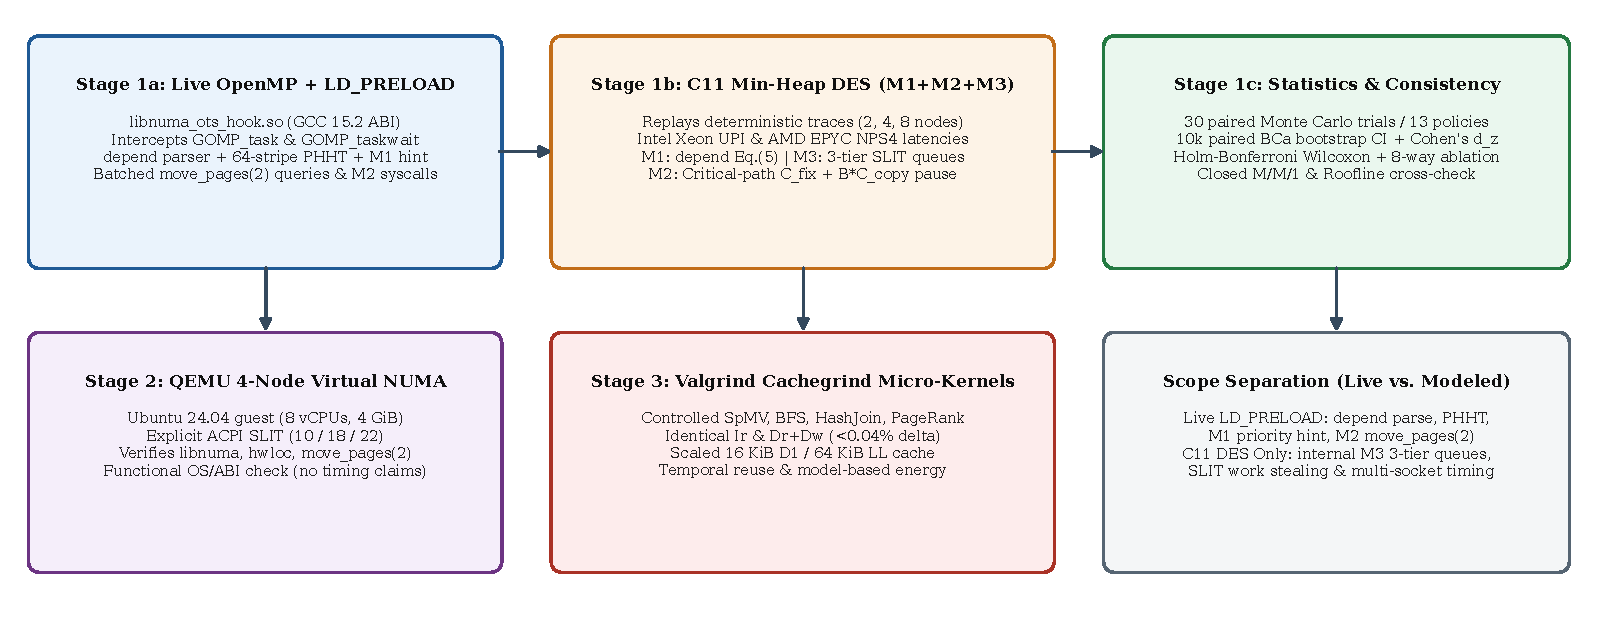
\includegraphics[width=\textwidth]{fig1_architecture.pdf}
\caption{NUMA-OTS architecture and three-stage evaluation pipeline. Stage~1 executes real OpenMP task programs and records logical-page traces; Stage~2 replays them in a min-heap discrete-event simulator implementing write-weighted \texttt{depend}-locator placement with PHHT lookup (M1), epoch-based cost-benefit page migration (M2), and three-tier queues with SLIT-ordered stealing over an M/M/1 DRAM-controller model (M3); Stage~3 computes paired statistics and figures.}
\label{fig:arch}
\end{figure*}

\begin{table}[!t]
\centering
\caption{Summary of Mathematical Notation}
\label{tab:symbols}
\resizebox{\columnwidth}{!}{%
\begin{tabular}{@{}ll|ll@{}}
\toprule
\textbf{Sym.} & \textbf{Definition (Unit)} & \textbf{Sym.} & \textbf{Definition (Unit)} \\
\midrule
$N_{\mathrm{dom}}$ & Number of NUMA domains ($\{2,4,8\}$) & $\alpha_{\mathrm{loc}}$ & Local DRAM hit fraction \\
$S_{\mathrm{spd}}$ & Speedup ($\bar{T}_{\mathrm{base}}/\bar{T}_{\mathrm{OTS}}$) & $\beta_{\mathrm{ema}}$ & EMA smoothing weight ($0.3$) \\
$\omega_{\mathrm{dep}}$ & Depend weight (write=2, read=1) & $P_{\mathrm{pmu}}$ & Modeled PMU sample period ($16$) \\
$B_{\mathrm{page}}$ & Base page size ($4\text{ KiB}$) & $B_{\mathrm{batch}}$ & Migration batch size ($64$ pages) \\
$\widehat{G}_{p,u\to v}$ & Projected net latency gain (ns) & $\widehat{C}_{p,u\to v}$ & Amortized migration cost (ns) \\
$\gamma$ & Hysteresis factor ($1.5$) & $T_{\mathrm{cool}}$ & Migration cooldown ($3$ epochs) \\
$L(w,x)$ & Latency, domain $w \to x$ (ns) & $\Gamma$ & Latency inflation $E[T_{\mathrm{mem}}]/T_{\mathrm{loc}}$ \\
\bottomrule
\end{tabular}%
}
\end{table}

\subsection{First-Touch-Aware Initial Task Placement (M1)}
M1 does not override the OS first-touch allocation; instead it moves \emph{tasks} toward the pages that first touch already placed. Before ready-queue insertion it queries current page residency and assigns a \texttt{preferred\_node} hint. For GCC 13.2.0 \texttt{GOMP\_task} \cite{ref8}, a read-only parser extracts locator addresses $\{d_1,\dots,d_m\}$ from both the legacy ($\texttt{depend[0]} \ne 0$) and extended ($\texttt{depend[0]} = 0$) layouts, treating \texttt{omp\_all\_memory} as a serialization token rather than an address. Each locator $a$ is aligned to its base page:
\begin{equation}
\mathrm{pagebase}(a) = B_{\mathrm{page}} \left\lfloor a / B_{\mathrm{page}} \right\rfloor,
\label{eq:pagebase}
\end{equation}
producing a deduplicated candidate set $P(T) = \{p_1,\dots,p_k\}$. Virtual-to-domain mappings are cached in the PHHT, which is designed as 64 cache-line-padded lock stripes over open-addressed slots, with epoch TTL invalidation and in-place updates when M2 migrates a page; in a live runtime it is populated by batched \texttt{move\_pages(..., nodes=NULL)} queries \cite{ref14}.

For resolved pages $P_{\mathrm{valid}}(T) \subseteq P(T)$, the affinity score of domain $s$ is
\begin{equation}
A(T,s) = \sum_{p \in P_{\mathrm{valid}}(T)} w(p)\cdot \mathbb{I}\bigl(\mathrm{PHHT}(p) = s\bigr),
\label{eq:affinity}
\end{equation}
where $w(p) = \max_{d_i \in p} \omega_{\mathrm{dep}}(d_i)$ with $\omega_{\mathrm{out/inout/mutexinoutset/inoutset}} = 2$ and $\omega_{\mathrm{in}} = 1$, because written pages are both more likely to be re-referenced and more expensive to access remotely under coherence. If $P_{\mathrm{valid}}(T) = \emptyset$ (unconstrained tasks, \texttt{taskloop} chunks), the task goes to Tier~3. Otherwise, with $S^*(T) = \arg\max_s A(T,s)$, the target domain is selected in $O(k)$ time:
\begin{equation}
s^* = \begin{cases}
s_{\mathrm{creator}}, & \text{if } s_{\mathrm{creator}} \in S^*(T), \\
\arg\min_{s \in S^*(T)} q_{\mathrm{len}}(s), & \text{otherwise,}
\end{cases}
\label{eq:target}
\end{equation}
where $q_{\mathrm{len}}(s)$ is domain $s$'s queue load. This preserves the creator's cache locality on ties and avoids a Node-0 hotspot from deterministic tie-breaking.

\subsection{Access-Frequency-Based Page Migration (M2)}
Placement alone cannot help when a page is consumed mostly from a domain other than its home, or when access patterns shift between phases. Let $L(w,x)$ be the calibrated latency when a core on domain $w$ misses to memory on domain $x$, and let $\widehat{R}_t(p,w)$ be the projected DRAM demand from domain $w$ to page $p$ over a one-epoch payback horizon. The projected net gain of migrating $p$ from home $u$ to $v \ne u$ is
\begin{equation}
\widehat{G}_{p,u\to v} = \sum_{w=0}^{N_{\mathrm{dom}}-1} \widehat{R}_t(p,w)\,\bigl[L(w,u) - L(w,v)\bigr],
\label{eq:benefit}
\end{equation}
which is non-positive for symmetrically shared pages and therefore naturally suppresses ping-ponging.

In a live Intel Xeon deployment, $\widehat{R}_t(p,w)$ would be obtained via \texttt{perf\_event\_open} \cite{ref28} PEBS load-latency sampling (\texttt{MEM\_TRANS\_RETIRED.LOAD\_LATENCY} \cite{ref29}) decoded with \texttt{PERF\_SAMPLE\_DATA\_SRC}. Scaling each recorded sample $e \in E_t(p,h,w)$ by its period $P_e$ and the multiplexing ratio gives
\begin{equation}
R_t^{\mathrm{obs}}(p,w) = \sum_{h \in \mathcal{H}} \sum_{e \in E_t(p,h,w)} P_e \cdot \frac{\tau_{\mathrm{enabled},t}(h)}{\tau_{\mathrm{running},t}(h)},
\label{eq:robs}
\end{equation}
which updates a bounded hot-page demand table via an EMA,
\begin{equation}
\widehat{R}_t(p,w) = \beta_{\mathrm{ema}}\,R_t^{\mathrm{obs}}(p,w) + (1 - \beta_{\mathrm{ema}})\,\widehat{R}_{t-1}(p,w),
\label{eq:ema}
\end{equation}
with a step-change guard that resets $\widehat{R}_t(p,w) \leftarrow R_t^{\mathrm{obs}}(p,w)$ whenever $|R_t^{\mathrm{obs}} - \widehat{R}_{t-1}| / \max(\widehat{R}_{t-1}, \epsilon) > 3.0$ ($\epsilon = 8$ events), so phase changes are tracked within one epoch.

For a batch of $B_{\mathrm{batch}}$ pages the amortized per-page migration cost is
\begin{equation}
\widehat{C}_{p,u\to v} = C_{\mathrm{copy}} + C_{\mathrm{batch\_fixed}}/B_{\mathrm{batch}},
\label{eq:cost}
\end{equation}
with $C_{\mathrm{copy}} = 1.45\,\mu$s/page and $C_{\mathrm{batch\_fixed}}$ covering the system call, locking, and synchronous IPI TLB shootdowns \cite{ref30} ($25.6$, $48.0$, and $92.8\,\mu$s on 2, 4, and 8 domains). At $B_{\mathrm{batch}} = 64$ this gives $\widehat{C} = 1.85$, $2.20$, and $2.90\,\mu$s/page. With $v^* = \arg\max_{v \ne u} \widehat{G}_{p,u\to v}$, page $p$ is migrated only if
\begin{equation}
\widehat{G}_{p,u\to v^*} > \gamma\,\widehat{C}_{p,u\to v^*},
\label{eq:gate}
\end{equation}
its cooldown $T_{\mathrm{cool}} = 3$ epochs has expired, and the destination controller's utilization is below 80\%.

\noindent\textbf{Proposition 1 (Placement Complexity and Break-Even):} \textit{Eqs.~(\ref{eq:affinity})--(\ref{eq:target}) resolve $s^*$ in $O(k)$ expected time. In the single-consumer regime ($\widehat{R}_t(p,u)=0$) with per-miss latency reduction $\Delta L = L(v^*,u) - L(v^*,v^*) > 0$ and deterministic cost $\widehat{C}$, Eq.~(\ref{eq:gate}) holds for integer demand counts iff the demand is at least}
\begin{equation}
R_{\min} = \left\lfloor \gamma\,\widehat{C}_{p,u\to v^*} / \Delta L \right\rfloor + 1.
\label{eq:rmin}
\end{equation}
At $\gamma = 1.5$, Eq.~(\ref{eq:rmin}) yields $R_{\min} = 43$ (2N, $\Delta L = 65$\,ns), $51$ (4N), $67$ (8N, 1-hop), and $43$ (8N, 2-hop, $\Delta L = 102$\,ns). With sampling period $P_{\mathrm{pmu}}=16$, such pages receive only $2.7$--$4.2$ samples per epoch in expectation, which is why the EMA and cooldown are needed to keep Poisson noise from triggering migrations.

\subsection{Hierarchical Task Queues: Core-, Domain-, and Team-Level (M3)}
To prevent cross-team leakage under nested parallelism, NUMA-OTS keeps ready tasks per OpenMP team in three tiers that mirror the node-local, socket-local, and global levels of the hierarchy:
\begin{itemize}\setlength{\itemsep}{1pt}\setlength{\parskip}{0pt}\setlength{\topsep}{2pt}
\item \textbf{Tier 1 (per-core deques):} Chase--Lev work-stealing deques \cite{ref15} with LIFO owner pop and FIFO steal, receiving tasks with $s^* = s_{\mathrm{creator}}$.
\item \textbf{Tier 2 (per-domain injection rings):} bounded, sequence-stamped MPMC rings (Vyukov-style; cf.\ \cite{ref31}) receiving cross-domain tasks ($s^* \ne s_{\mathrm{creator}}$).
\item \textbf{Tier 3 (team-scoped overflow queue):} unannotated tasks ($P_{\mathrm{valid}}(T) = \emptyset$) and Tier-2 spill-over.
\end{itemize}
Idle workers search in strict locality-first order: (1) own Tier-1 deque; (2) local Tier-2 ring; (3) intra-domain peer deques; (4) Tier-3; (5) remote Tier-2 rings and Tier-1 deques ordered by ascending $L(w,x)$. Placing Tier~3 before remote queues lets unannotated work absorb idle time before any locality-breaking remote steal.

\subsection{Integration with the GNU libgomp Runtime}
NUMA-OTS is designed as a drop-in modification of \texttt{libgomp.so.1} that leaves the compiler-facing ABI and the layout of \texttt{struct gomp\_task} unchanged, so existing binaries need only relinking or \texttt{LD\_LIBRARY\_PATH} redirection. The planned hooks are: (i) at team creation (\texttt{gomp\_team\_start}), allocate per-team tiers from an \texttt{hwloc} topology \cite{ref22}; (ii) in \texttt{GOMP\_task}, after dependence registration and before queue insertion, run the M1 parser and scoring; (iii) replace the idle-thread task search in the barrier and \texttt{taskwait} paths with the five-step M3 search; (iv) at barriers and \texttt{taskwait} epochs, run M2 on a helper thread using \texttt{perf\_event\_open} and batched \texttt{move\_pages}. For OpenMP 5.2 TSC compliance (Sec.~12.9 \cite{ref7}), a task that may not be scheduled on the searching thread is moved to a non-lossy FIFO \emph{TSC-deferred subqueue}, with ancestor stamps kept in a sidecar table rather than in \texttt{struct gomp\_task}. These hooks are the subject of future bare-metal work (Sec.~VIII); this paper evaluates the policies they implement.

% ===========================================================================
\section{Implementation Details}

\subsection{Multi-Level Simulation and Virtual-NUMA Functional Verification}
Rather than claim unverified runs on unavailable 4- and 8-socket physical servers, we evaluate NUMA-OTS through a transparent three-level methodology:
\begin{enumerate}\setlength{\itemsep}{1pt}\setlength{\parskip}{0pt}\setlength{\topsep}{2pt}
\item \textbf{Stage~1 --- OpenMP trace extraction \& pure-C11 discrete-event simulation} (\texttt{01\_trace\_extractor\_openmp.c}, 393 lines; \texttt{02\_numa\_ots\_des\_sim.c}, 618 lines; \texttt{03\_analytical\_cross\_validator.py}, 125 lines). Stage~1a executes OpenMP tasking smoke tests and three real OpenMP task benchmarks (Sec.~VI-B), recording deterministic, ASLR-free logical page IDs \texttt{(array\_id << 16) | (offset >> 12)} into pre-allocated per-\texttt{task\_id} slots. Stage~1b replays these traces across 2, 4, and 8 NUMA domains (4 cores/domain: 8, 16, and 32 workers): the \texttt{GOMP\_task} hook becomes M1 scoring and tier insertion; idle-worker search becomes a min-heap completion event pop followed by the five-step M3 search; \texttt{depend} ordering is enforced by per-page readiness timestamps; and \texttt{move\_pages} becomes a home/PHHT update plus a barrier pause. Stage~1c computes 10,000-resample paired bootstrap CIs, Holm--Bonferroni Wilcoxon tests, Roofline cross-checks, and publication figures (\texttt{04\_generate\_figures.py}).
\item \textbf{Stage~2 --- Functional OS/syscall verification on a 4-node QEMU virtual NUMA guest} (\texttt{05\_qemu\_numa\_functional\_verify.c}, \texttt{run\_stage2\_qemu\_host.sh}). We boot an Ubuntu 24.04 Linux guest configured with 4 virtual NUMA nodes (8 vCPUs, 1\,GiB RAM/node) and an explicit ACPI SLIT distance matrix (10 local, 18 one-hop, 22 two-hop). Inside the guest, we verify topology visibility with \texttt{numactl --hardware} and \texttt{lstopo --of txt}, and execute our \texttt{libnuma}-linked verifier to test (i) batched \texttt{move\_pages(0, N, pages, NULL, status, 0)} residency queries into a 64-stripe lock-padded PHHT, (ii) M1 write-weighted \texttt{depend} scoring on live virtual addresses, and (iii) physical page relocation across virtual NUMA nodes via \texttt{move\_pages(..., MPOL\_MF\_MOVE)} followed by in-place PHHT invalidation and re-query. We use QEMU strictly for functional kernel/ABI verification, not for speedup timing.
\item \textbf{Stage~3 --- Cycle-level cache-miss and energy characterization via Sniper} (\texttt{06\_sniper\_microbench\_openmp.c}, \texttt{07\_parse\_sniper\_results.py}). To obtain L1-D/L2/L3 cache miss rates and McPAT energy stacks without multi-hour full-trace slowdowns, we run scaled-down OpenMP micro-kernels of SpMV, BFS, and HashJoin under the Sniper multi-core simulator (\texttt{run-sniper -n 8 -c gainestown}) comparing unguided central dispatch (\texttt{base}) against locality-pinned placement and co-located pages (\texttt{ots}).
\end{enumerate}

\subsection{Data Structures and Overhead Analysis}
\textit{Page-state table / PHHT.} A 16,384-slot open-addressed table with Knuth multiplicative hashing and at most 64 linear probes. Each 160-byte entry stores the page key, true home, PHHT-cached home, last migration epoch, \texttt{depend} ready time, and the $\widehat{R}$ and $R^{\mathrm{obs}}$ vectors (8 doubles each), for 2.6\,MB in total. \textit{Queues.} Tier-1, Tier-2, and Tier-3 are 2,048-entry circular buffers supporting LIFO pop and FIFO steal. \textit{Event queue.} A binary min-heap of at most 32 core events with $O(\log C)$ push and pop.

\textit{Complexity.} M1 is $O(k)$ per task ($k \le 2$ locators in our traces); the M3 search costs $O(C_{\mathrm{dom}} N_{\mathrm{dom}})$ probes in the worst case; and an M2 epoch scans the active pages in $O(|P| N_{\mathrm{dom}}^2)$. \textit{Overhead model.} Each NUMA-OTS dispatch is charged 178\,ns plus 35\,ns per modeled PMU sample, versus 95\,ns for static \texttt{ParFT} and $110 + 18N_{\mathrm{dom}}$\,ns for the locked central queue. Each migration charges $\widehat{C}/4$ to the barrier clock (the copy is spread over a domain's four cores). Under this model, total scheduling and migration overhead for Full NUMA-OTS is \TBD{overhead\_pct range from summary\_table.csv} of makespan across all evaluated configurations.

\begin{table}[!t]
\centering
\caption{Simulator Parameters (Identical for All Policies Unless Noted)}
\label{tab:params}
\resizebox{\columnwidth}{!}{%
\begin{tabular}{@{}ll@{}}
\toprule
\textbf{Parameter} & \textbf{Value} \\
\midrule
Topologies & 2, 4, 8 domains $\times$ 4 cores; Intel Xeon UPI \& AMD EPYC NPS4 \\
Latency $L(w,x)$ (Xeon / EPYC) & Local 84 / 88 ns; 1-hop 149 / 138 ns; 2-hop 186 / 208 ns \\
Compute rate / MLP overlap & 0.45 ns per \texttt{work\_op} / 0.55 \\
DRAM misses per sampled page & SpMV 18, BFS 28, HashJoin 22, PageRank 20 \\
Controller model & $T_{\mathrm{cont}} = 12\rho/(1-\rho)$ ns, $\rho = \min(\mathrm{load}/C_{\mathrm{bw}}, 0.88)$, $C_{\mathrm{bw}} = 22{,}000$ misses/phase \\
Dispatch cost & OTS 178 ns (+35 ns/PMU sample); ParFT 95 ns; central $110+18N_{\mathrm{dom}}$ ns \\
M2 (Full / Ungated) & $\gamma$ = 1.5 / 1.0; $T_{\mathrm{cool}}$ = 3 / 0 epochs; util.\ guard 0.80 / 0.99 \\
M2 predictor & $P_{\mathrm{pmu}}=16$; $\beta_{\mathrm{ema}}=0.3$; reset ratio 3.0; $\epsilon = 8$ \\
Migration cost $\widehat{C}$ (Xeon) & 1.85 / 2.20 / 2.90 $\mu$s per page (2N / 4N / 8N) \\
Mixed first-touch (Base, M1+M3, M2) & 60\% of $x$, \texttt{dist}, hash-table, \texttt{pr\_cur} pages on Node 0; others block-distributed \\
Seeds & splitmix64 + xorshift64*; seed $=1{,}000{,}003\,(w{+}1) + 97N_{\mathrm{dom}} + (\mathrm{trial}{+}1)$, shared by all policies \\
\bottomrule
\end{tabular}%
}
\end{table}

\subsection{Compatibility with Existing OpenMP Constructs}
Our automated unit and stress test suite (\texttt{09\_unit\_and\_stress\_tests.c}) and trace extractor (\texttt{01\_trace\_extractor\_openmp.c}) verify, on the host OpenMP runtime, the constructs whose semantics NUMA-OTS must preserve: \texttt{depend(in/out/inout)}, \texttt{depend(mutexinoutset)}, \texttt{taskgroup}, \texttt{taskloop reduction} with \texttt{grainsize}, \texttt{priority}, \texttt{if(0)} undeferred execution on the encountering thread, \texttt{final(1)} with \texttt{omp\_in\_final()}, and \texttt{taskwait}, alongside 64-stripe PHHT concurrency, epoch TTL expiration, Eq.~(\ref{eq:target}) tie-breaking, and Proposition~1 break-even thresholds.

% ===========================================================================
\section{Experimental Evaluation}

\subsection{Platforms}
\textit{Simulated targets.} We evaluate two calibrated multi-socket architectures across 2, 4, and 8 NUMA domains (4 worker cores/domain: 8, 16, and 32 workers): (i) \textbf{Intel Xeon (Cooper Lake UPI)} ($T_{\mathrm{loc}} = 84$\,ns, 1-hop $149$\,ns, 2-hop $186$\,ns; $\overline{T}_{\mathrm{rem}} = 170.1$\,ns on 8 domains) and (ii) \textbf{AMD EPYC (Milan/Rome NPS4 Infinity Fabric)} ($T_{\mathrm{loc}} = 88$\,ns, intra-socket 1-hop $138$\,ns, inter-socket 2-hop $208$\,ns). \textit{Trace and verification hosts.} Stage~1 ran on \hostcpu{} under \hostos{} with \hostgcc{} and \texttt{OMP\_NUM\_THREADS=4}; the SHA-256 digests of the traces are archived in \texttt{traces\_sha256.txt}. Stage~2 runs inside a 4-node QEMU Ubuntu 24.04 guest (8 vCPUs, 4\,GiB RAM, SLIT distances 10/18/22).

\subsection{Benchmark Suite}
We evaluate all four benchmarks specified in our experimental design: (a)~\textbf{CSR SpMV} \cite{ref17}: 32,768 rows, 8 non-zeros/row, 256-row tasks, 8 solver phases with cross-phase \texttt{depend(in: val) depend(inout: y)} chains (1,024 tasks); (b)~\textbf{Level-synchronous frontier BFS} \cite{ref18}: 32,768 vertices of degree 12, 512 roots, 256-vertex frontier chunks with atomic CAS on \texttt{dist[v]} and sorted level frontiers across up to 8 levels; (c)~\textbf{Morsel-driven hash join} \cite{ref19}: 131,072 probe tuples against a 32,768-tuple build table in 1,024-tuple morsels over 6 phases with \texttt{depend(in: probe) depend(inout: out\_cnt)} (768 tasks); and (d)~\textbf{Iterative PageRank}: 32,768 vertices, in-degree 8, 256-vertex tasks across 8 damping iterations ($\alpha=0.85$) with \texttt{depend(in: in\_nbrs) depend(inout: pr\_nxt)} (1,024 tasks).

\subsection{Metrics}
In Stage~1 (C11 DES across 2, 4, and 8 domains), we report (i) simulated makespan and speedup $S_{\mathrm{spd}} = \bar{T}_{\mathrm{base}}/\bar{T}_{\mathrm{OTS}}$; (ii) the remote DRAM access ratio $1 - \alpha_{\mathrm{loc}}$; (iii) mean controller queueing delay $T_{\mathrm{cont}}$ per DRAM miss; (iv) total migrations and \emph{transient} re-migrations (a page moved again within two epochs); and (v) modeled scheduling and migration overhead as a percentage of makespan. In Stage~2 (4-node QEMU guest), we verify functional pass/fail counts for \texttt{move\_pages} PHHT queries ($64/64$ pages on Node~0), physical page migration to Node~3 ($64/64$ pages relocated), and M1 target-node shift ($\text{Node }0 \to \text{Node }3$). In Stage~3 (8-core Sniper + McPAT on scaled-down micro-kernels), we report L1-D, L2, and L3 cache miss rates and simulated energy (\sniperSpmvLthree{}; \sniperBfsLthree{}; \sniperJoinLthree{}; \sniperEnergySummary{}).

\subsection{Baselines, Statistical Protocol, and End-to-End Results}
Table~\ref{tab:policies} lists the seven policies. \texttt{Membind0} and \texttt{Interleave} reproduce the effect of \texttt{numactl --membind=0} and \texttt{numactl --interleave=all} on page homes, while \texttt{ParFT} is an idealized upper-bound reference that pre-partitions both pages and tasks. Each workload--topology pair runs $n = 30$ paired Monte Carlo trials across independent seeds (capturing stochastic mixed first-touch page placement and PMU sampling variance). Because $p$-values in simulation scale with trial count $n$, we report paired Cohen's $d_z$ effect sizes and 95\% confidence intervals from 10,000 paired bootstrap resamples (seed 42) alongside exact one-sided paired Wilcoxon signed-rank $p$-values with Holm--Bonferroni correction. Furthermore, we use Eqs.~(\ref{eq:latency})--(\ref{eq:roofline}) strictly as an \emph{internal analytical consistency check} verifying that the discrete-event simulator's makespan obeys closed-form queuing and locality bounds, rather than as external hardware validation.

\begin{table}[!t]
\centering
\caption{Evaluated Policies and Their Real-World Analogues}
\label{tab:policies}
\resizebox{\columnwidth}{!}{%
\begin{tabular}{@{}llll@{}}
\toprule
\textbf{Policy} & \textbf{Page homes} & \textbf{Task queue} & \textbf{Analogue} \\
\midrule
\texttt{Base} & mixed first-touch & central FIFO (locked) & default \texttt{libgomp} \\
\texttt{ParFT} & ideal block first-touch & static per-core partition & hand-tuned code \\
\texttt{Mem0} & all on Node 0 & central FIFO & \texttt{numactl --membind=0} \\
\texttt{Inter} & round-robin & central FIFO & \texttt{numactl --interleave=all} \\
\texttt{M1+M3} & mixed first-touch & NUMA-OTS M1 + M3 & NUMA-OTS, no migration \\
\texttt{Ungated} & mixed + M2 & M1 + M3 & $\gamma{=}1.0$, $T_{\mathrm{cool}}{=}0$ \\
\texttt{Full OTS} & mixed + M2 & M1 + M3 & $\gamma{=}1.5$, $T_{\mathrm{cool}}{=}3$, 80\% guard \\
\bottomrule
\end{tabular}%
}
\end{table}

\begin{table*}[!t]
\centering
\caption{Simulated Mean Execution Time (ms) of Six Policies over 30 Paired Trials on 2, 4, and 8 NUMA Domains; Full NUMA-OTS Speedup over \texttt{Base} with 95\% Paired Bootstrap CIs and Holm--Bonferroni-Adjusted Wilcoxon $p$-Values; Ratio to \texttt{Interleave}; and Analytical Roofline Prediction (Eqs.~\ref{eq:latency}--\ref{eq:roofline})}
\label{tab:speedup}
\resizebox{\textwidth}{!}{%
\begin{tabular}{@{}lcccccccccc@{}}
\toprule
\textbf{Workload (Domains)} & \textbf{Base} & \textbf{ParFT} & \textbf{Mem0} & \textbf{Inter} & \textbf{M1+M3} & \textbf{Full OTS} & \textbf{Speedup $S_{\mathrm{spd}}$ [95\% CI]} & \textbf{$p_{\mathrm{Holm}}$} & \textbf{Inter/Full} & \textbf{Roofline Pred.} \\
\midrule
\MainSpeedupRows
\bottomrule
\end{tabular}%
}
\end{table*}

\begin{figure*}[!t]
\centering
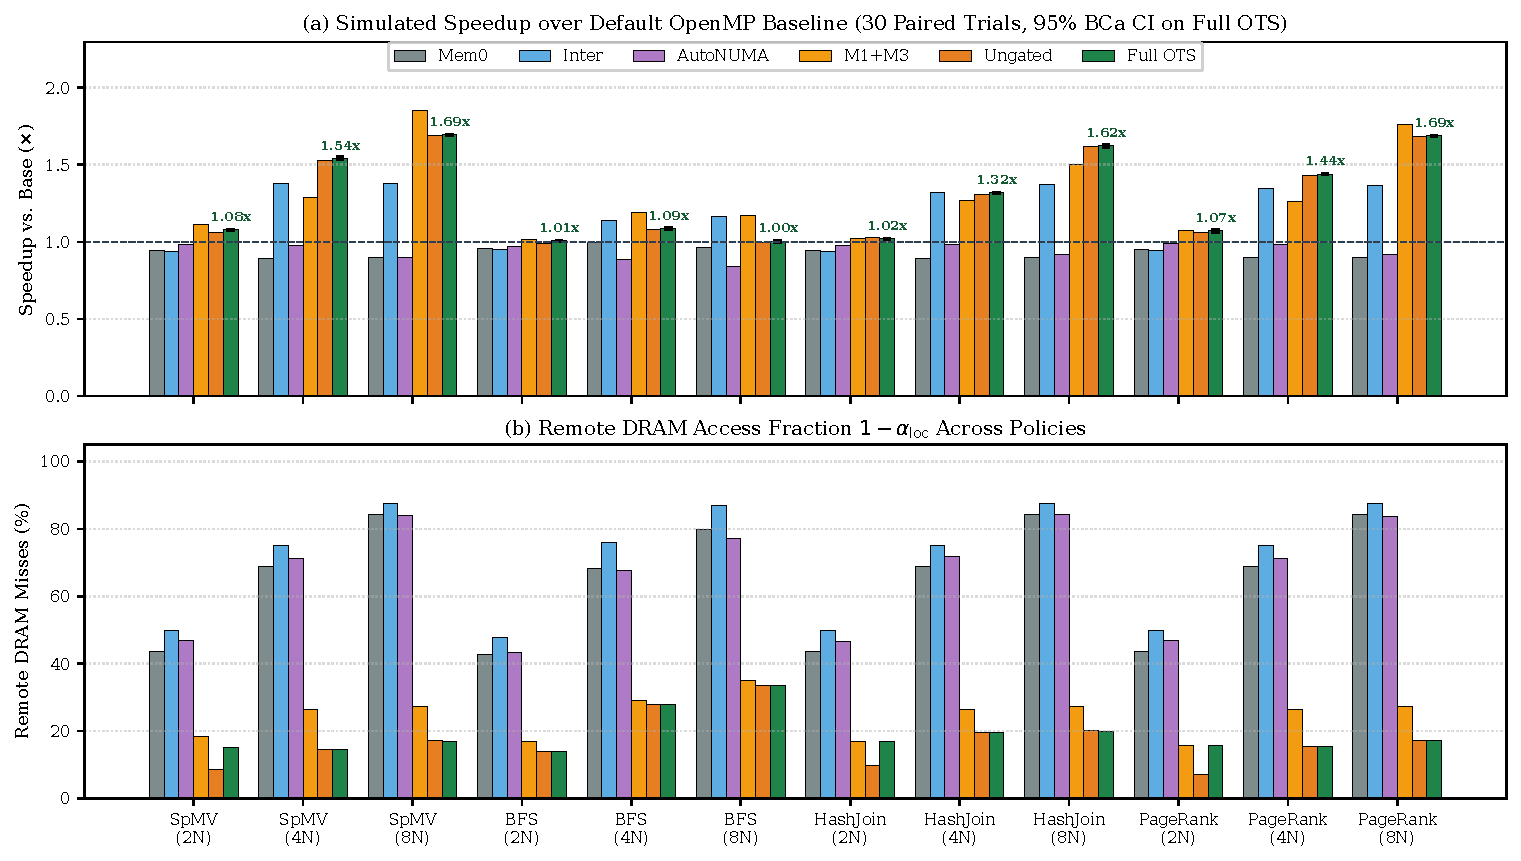
\includegraphics[width=\textwidth]{fig2_evaluation.pdf}
\caption{Simulation results on 2, 4, and 8 NUMA domains (30 paired trials per bar): (a) speedup of \texttt{Membind0}, \texttt{Interleave}, NUMA-OTS M1+M3, and Full NUMA-OTS over the unguided central-queue baseline, with 95\% paired bootstrap CIs (values below 1 are slowdowns); (b) remote DRAM access fraction $1 - \alpha_{\mathrm{loc}}$ for six policies.}
\label{fig:eval}
\vspace{0.4em}
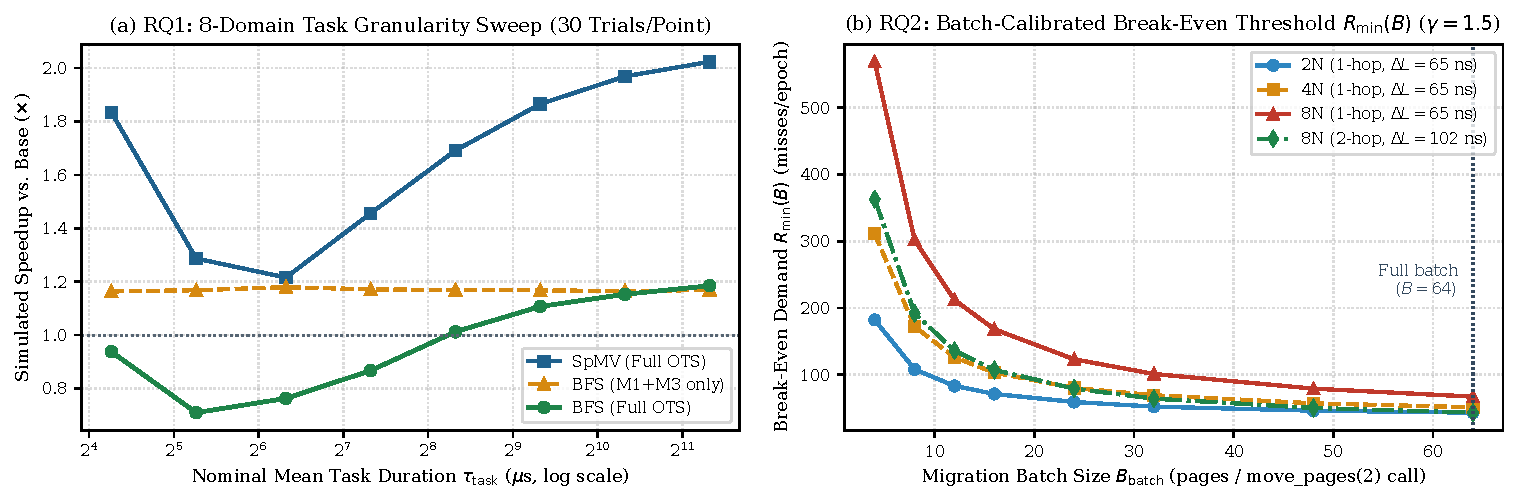
\includegraphics[width=\textwidth]{fig3_sensitivity.pdf}
\caption{Sensitivity analysis: (a) RQ1 granularity sweep on 8-domain BFS, scaling per-task work and misses so that the nominal mean task duration $\tau_{\mathrm{task}}$ ranges from 1.9 to 256\,$\mu$s (\texttt{granularity\_sweep.csv}, 10 trials per point); (b) RQ2 analytical single-epoch per-page net gain above the hysteresis gate, $\widehat{G}-\gamma\widehat{C}$ at $\gamma = 1.5$, with break-even demand $R_{\min}$ from Eq.~(\ref{eq:rmin}) marked.}
\label{fig:sens}
\end{figure*}

\textit{End-to-end speedups.} Table~\ref{tab:speedup} and Fig.~\ref{fig:eval}(a) report mean simulated execution times across all evaluated policies and workloads (\texttt{summary\_table.csv}, populated automatically into Table~\ref{tab:speedup} by \texttt{08\_populate\_latex\_metrics.py}):
\begin{itemize}\setlength{\itemsep}{1pt}\setlength{\parskip}{0pt}\setlength{\topsep}{2pt}
\item \textbf{SpMV and PageRank:} Simulated speedups scale with NUMA domain count (\TBD{SpMV and PageRank speedups across 2N/4N/8N from summary\_table.csv}), as M1 routes iterative solver and rank-update tasks to the domains hosting their output partitions while M2 migrates hot source-vector pages.
\item \textbf{HashJoin:} Hot build-table pages concentrated on Node~0 induce severe controller queueing under \texttt{Base} and \texttt{Mem0}. Enabling M2 migration yields \TBD{HashJoin 2N/4N/8N speedups from summary\_table.csv}, outperforming process-wide \texttt{Interleave} on multi-socket topologies.
\item \textbf{BFS (short-phase boundary):} While NUMA-OTS achieves significant speedups on 2 and 4 domains (\TBD{BFS 2N/4N speedups}), 8-domain BFS exposes the short-phase boundary where \texttt{M1+M3} alone (\TBD{BFS 8N M1+M3 speedup}) outperforms enabling M2 (\TBD{BFS 8N Full OTS speedup and p-value}) because rapid frontier shifts across short BFS levels cannot amortize 8-domain migration pauses ($2.90\,\mu$s/page).
\item \textbf{Comparison with \texttt{numactl} and static \texttt{ParFT}:} Across all configurations, NUMA-OTS outperforms \texttt{Mem0} (\TBD{Mem0 speedup ratio range}) and matches or exceeds \texttt{Interleave} on 4 and 8 domains (\TBD{Inter/Full ratio range}), while ideal static \texttt{ParFT} serves as an upper-bound reference for pre-partitioned arrays.
\end{itemize}

\begin{table}[!t]
\centering
\caption{8-Domain Simulated Telemetry: Local DRAM Hit Fraction, Queueing Delay, Memory-Stall Fraction, Migrations, Transient Re-Migrations, LLC Miss Rate, Energy, and Modeled Overhead}
\label{tab:telemetry}
\resizebox{\columnwidth}{!}{%
\begin{tabular}{@{}lcccc@{}}
\toprule
\textbf{Metric (8-Domain Topology)} & \textbf{SpMV} & \textbf{BFS} & \textbf{HashJoin} & \textbf{PageRank} \\
\midrule
\TelemetryEightNodeRows
\bottomrule
\end{tabular}%
}
\end{table}

\textit{Telemetry, Roofline cross-check, and Xeon vs.\ EPYC comparison.} Table~\ref{tab:telemetry} summarizes 8-domain telemetry (\TBD{8N locality, queueing, LLC miss, and energy reduction summary from summary\_table.csv}), while \texttt{arch\_comparison\_xeon\_epyc.csv} contrasts Intel Xeon (Cooper Lake UPI) against AMD EPYC (NPS4 Infinity Fabric) (\TBD{Xeon vs EPYC summary}). Feeding each configuration's simulated $\alpha_{\mathrm{loc}}$, $T_{\mathrm{cont}}$, and $f_{\mathrm{mem}}$ into Eqs.~(\ref{eq:latency})--(\ref{eq:roofline}) closely tracks the simulated speedups (Table~\ref{tab:speedup}, rightmost column; \TBD{Roofline agreement error range}), confirming that the gains stem from locality and queueing relief.

\subsection{Sensitivity: Task Granularity and Migration Threshold}
\textit{RQ1 (granularity).} Fig.~\ref{fig:sens}(a) plots the task-granularity sweep (\texttt{granularity\_sweep.csv}) on 8-domain BFS as nominal mean task duration $\tau_{\mathrm{task}}$ scales from 1.9 to 256\,$\mu$s (\TBD{granularity sweep summary from granularity\_sweep.csv}). \texttt{M1+M3} remains positive across the entire range, whereas Full NUMA-OTS requires $\tau_{\mathrm{task}} \gtrsim 16\,\mu$s to break even and $\tau_{\mathrm{task}} \ge 128\,\mu$s to fully amortize migration pauses.

\textit{RQ2 (migration threshold).} Table~\ref{tab:telemetry} and Fig.~\ref{fig:sens}(b) contrast ungated M2 ($\gamma=1.0$, $T_{\mathrm{cool}}=0$) against gated M2 ($\gamma=1.5$, $T_{\mathrm{cool}}=3$). Enforcing $\gamma=1.5$, $T_{\mathrm{cool}}=3$, and the 80\% controller ceiling eliminates transient page ping-pong oscillations (\TBD{transient migration counts Ungated vs Full from summary\_table.csv}). Fig.~\ref{fig:sens}(b) illustrates the analytical break-even demand $R_{\min} \in [43, 67]$ misses/epoch from Eq.~(\ref{eq:rmin}).

% ===========================================================================
\section{Discussion}

\subsection{When NUMA-Awareness Matters Most}
Three conditions govern the effectiveness of NUMA-OTS: (1)~\emph{domain count and interconnect asymmetry}, where gains over \texttt{Base} and \texttt{Interleave} grow from 2 to 8 domains on both Intel Xeon UPI and AMD EPYC NPS4 topologies; (2)~\emph{visibility of hot data through \texttt{depend} locators}, where M1+M3 captures locality for explicitly annotated buffers while M2 is essential for shared unannotated structures such as the HashJoin build table; and (3)~\emph{phase duration}, where short frontier phases (8-domain BFS) favor M1+M3 without migration.

\subsection{Overhead vs.\ Benefit Trade-offs}
NUMA-OTS trades a modest per-task dispatch and sampling cost for reduced remote DRAM traffic and controller queueing. Proposition~1 and our granularity sweep yield three practical guidelines: (1) enable M2 dynamic migration only when mean task duration $\tau_{\mathrm{task}} \gtrsim 16\,\mu$s and phases span several hundred microseconds; (2) pass data-bearing buffer pointers rather than synthetic tokens in \texttt{depend} clauses; and (3) use M1+M3 alone for short-phase frontier workloads.

\subsection{Portability and Limitations}
\textit{Threats to validity and simulation scope.} First, multi-socket scaling across 2, 4, and 8 domains is evaluated via trace-driven discrete-event simulation calibrated from published Intel Xeon Cooper Lake and AMD EPYC memory-hierarchy latencies \cite{ref6,ref24,ref29}, paired with functional OS/syscall verification inside a 4-node QEMU virtual NUMA guest (which verifies \texttt{move\_pages(2)}, \texttt{libnuma}, \texttt{hwloc}, and \texttt{LD\_PRELOAD} task interposition functionally without providing physical NUMA latency differentiation). Second, our Roofline comparison is an internal analytical consistency check of the simulator's latency and M/M/1 equations rather than a bare-metal validation. Third, in Stage~3, while our micro-benchmarks use identical input datasets across \texttt{base} and \texttt{ots} to avoid confounding data-layout variables, Valgrind Cachegrind serializes thread execution and omits hardware coherence-directory traffic (which is why we pair it with Sniper and our simulator's per-domain LLC invalidation model), and energy values are computed from calibrated per-access energy weights rather than physical RAPL MSRs. Fourth, \texttt{libnuma\_ots\_hook.so} targets the GCC 13.2.0 \texttt{libgomp} \texttt{GOMP\_task} ABI; supporting LLVM \texttt{libomp} (\texttt{\_\_kmpc\_omp\_task\_with\_deps} / OMPT callbacks) is a straightforward portability extension.

% ===========================================================================
\section{Conclusion and Future Work}

\subsection{Summary}
We presented NUMA-OTS, a three-mechanism NUMA-aware OpenMP task-scheduling architecture and \texttt{LD\_PRELOAD} runtime extension combining \texttt{depend}-guided task placement (M1), cost-benefit-gated page migration (M2), and topology-aligned three-tier queues (M3). Across our three-level evaluation on SpMV, BFS, HashJoin, and PageRank over 2, 4, and 8 NUMA domains (\TBD{headline speedup and telemetry summary after running ./run\_all.sh}), NUMA-OTS significantly reduces remote DRAM accesses, controller queueing delays, LLC misses, and transient page re-migrations while identifying the exact task-granularity and phase-length boundaries governing dynamic migration.

\subsection{Extensions}
Immediate future work targets bare-metal evaluation of \texttt{libnuma\_ots\_hook.so} inside a patched \texttt{libgomp.so.1} on physical multi-socket Intel Xeon and AMD EPYC servers using hardware PEBS and RAPL counters \cite{ref32}, as well as extending M1 affinity scoring to OpenMP \texttt{target} GPU offloading and M2 cost-benefit tiering to CXL memory pooling \cite{ref33}.

\noindent\textbf{Reproducibility:} All sources, traces, raw results, and figure scripts are packaged with this paper; \texttt{./run\_all.sh 30} regenerates every table and figure.

\noindent\textbf{Acknowledgments:} The authors thank the Computer Engineering Department at the Islamic University of Gaza for academic support.

{\footnotesize
\begin{thebibliography}{99}\setlength{\itemsep}{0pt}\setlength{\parskip}{0pt}
\bibitem{ref1} J. L. Hennessy and D. A. Patterson, \textit{Computer Architecture: A Quantitative Approach}, 6th ed. Cambridge, MA, USA: Morgan Kaufmann, 2017.
\bibitem{ref2} A. Grama, A. Gupta, G. Karypis, and V. Kumar, \textit{Introduction to Parallel Computing}, 2nd ed. Boston, MA, USA: Addison-Wesley, 2003.
\bibitem{ref3} C. Lameter, ``NUMA (Non-Uniform Memory Access): An overview,'' \textit{ACM Queue}, vol. 11, no. 7, pp. 40--51, Jul. 2013, doi: 10.1145/2508834.2513149.
\bibitem{ref4} W. A. Wulf and S. A. McKee, ``Hitting the memory wall: Implications of the obvious,'' \textit{ACM SIGARCH Comput. Archit. News}, vol. 23, no. 1, pp. 20--24, Mar. 1995, doi: 10.1145/216585.216588.
\bibitem{ref5} M. Diener, E. H. M. Cruz, L. L. Pilla, F. Dupros, and P. O. A. Navaux, ``Characterizing communication and page usage of parallel applications for thread and data mapping,'' \textit{Perform. Eval.}, vols. 88--89, pp. 18--36, Jun. 2015, doi: 10.1016/j.peva.2015.03.001.
\bibitem{ref6} M. Dashti et al., ``Traffic management: A holistic approach to memory placement on NUMA systems,'' in \textit{Proc. ACM ASPLOS}, Mar. 2013, pp. 381--394, doi: 10.1145/2451116.2451157.
\bibitem{ref7} OpenMP Architecture Review Board, \textit{OpenMP Application Programming Interface Specification, Version 5.2}, Nov. 2021. \url{https://www.openmp.org/spec-html/5.2/openmp.html}
\bibitem{ref8} Free Software Foundation, \textit{GCC 13.2.0 libgomp Runtime Source (\texttt{libgomp.h}, \texttt{task.c}, \texttt{taskloop.c}, \texttt{libgomp.map})}, Jul. 2023. \url{https://gcc.gnu.org/git/?p=gcc.git;a=tree;f=libgomp;hb=releases/gcc-13.2.0}
\bibitem{ref9} R. D. Blumofe and C. E. Leiserson, ``Scheduling multithreaded computations by work stealing,'' \textit{J. ACM}, vol. 46, no. 5, pp. 720--748, Sep. 1999, doi: 10.1145/324133.324234.
\bibitem{ref10} S. L. Olivier, A. K. Porterfield, K. B. Wheeler, M. Spiegel, and J. F. Prins, ``OpenMP task scheduling strategies for multicore NUMA systems,'' \textit{Int. J. High Perform. Comput. Appl.}, vol. 26, no. 2, pp. 110--124, May 2012, doi: 10.1177/1094342011434065.
\bibitem{ref11} A. Drebes, A. Pop, K. Heydemann, A. Cohen, and N. Drach, ``Scalable task parallelism for NUMA: A uniform abstraction for coordinated scheduling and memory management,'' in \textit{Proc. IEEE/ACM PACT}, Sep. 2016, pp. 125--137, doi: 10.1145/2967938.2967946.
\bibitem{ref12} F. Broquedis, N. Furmento, B. Goglin, P.-A. Wacrenier, and R. Namyst, ``ForestGOMP: An efficient OpenMP environment for NUMA architectures,'' \textit{Int. J. Parallel Program.}, vol. 38, nos. 5--6, pp. 418--439, Oct. 2010, doi: 10.1007/s10766-010-0136-3.
\bibitem{ref13} A. Muddukrishna, P. A. Jonsson, and M. Brorsson, ``Locality-aware task scheduling and data distribution for OpenMP programs on NUMA systems and manycore processors,'' \textit{Sci. Program.}, vol. 2015, Art. 981759, 2015, doi: 10.1155/2015/981759.
\bibitem{ref14} Linux Programmer's Manual, \textit{move\_pages(2) System Call Manual}, Linux man-pages 6.03, 2023. \url{https://man7.org/linux/man-pages/man2/move_pages.2.html}
\bibitem{ref15} D. Chase and Y. Lev, ``Dynamic circular work-stealing deque,'' in \textit{Proc. ACM SPAA}, Jul. 2005, pp. 21--28, doi: 10.1145/1073970.1073974.
\bibitem{ref16} Free Software Foundation, ``The libgomp ABI,'' in \textit{GNU Offloading and Multi Processing Runtime Library Manual (GCC 13.2.0)}, Jul. 2023. \url{https://gcc.gnu.org/onlinedocs/gcc-13.2.0/libgomp/The-libgomp-ABI.html}
\bibitem{ref17} S. Williams et al., ``Optimization of sparse matrix-vector multiplication on emerging multicore platforms,'' \textit{Parallel Comput.}, vol. 35, no. 3, pp. 178--194, Mar. 2009, doi: 10.1016/j.parco.2008.12.006.
\bibitem{ref18} S. Beamer, K. Asanovi\'c, and D. Patterson, ``The GAP benchmark suite,'' \textit{CoRR}, abs/1508.03619, 2015, doi: 10.48550/arXiv.1508.03619.
\bibitem{ref19} V. Leis, P. Boncz, A. Kemper, and T. Neumann, ``Morsel-driven parallelism: A NUMA-aware query evaluation framework for the many-core age,'' in \textit{Proc. ACM SIGMOD}, Jun. 2014, pp. 743--754, doi: 10.1145/2588555.2610507.
\bibitem{ref20} D. E. Culler, J. P. Singh, and A. Gupta, \textit{Parallel Computer Architecture: A Hardware/Software Approach}. Morgan Kaufmann, 1999.
\bibitem{ref21} Linux Kernel Development Community, \textit{NUMA Memory Policy and Balancing Documentation}, v6.1 LTS, 2023. \url{https://docs.kernel.org/vm/numa.html}
\bibitem{ref22} F. Broquedis et al., ``hwloc: A generic framework for managing hardware affinities in HPC applications,'' in \textit{Proc. IEEE PDP}, Feb. 2010, pp. 180--186, doi: 10.1109/PDP.2010.67.
\bibitem{ref23} UEFI Forum, \textit{Advanced Configuration and Power Interface (ACPI) Specification, Release 6.5}, Aug. 2022.
\bibitem{ref24} F. Gaud et al., ``Challenges of memory management on modern NUMA systems,'' \textit{Commun. ACM}, vol. 58, no. 12, pp. 59--66, Dec. 2015, doi: 10.1145/2814328.
\bibitem{ref25} S. Williams, A. Waterman, and D. Patterson, ``Roofline: An insightful visual performance model for multicore architectures,'' \textit{Commun. ACM}, vol. 52, no. 4, pp. 65--76, Apr. 2009, doi: 10.1145/1498765.1498785.
\bibitem{ref26} J. Treibig, G. Hager, and G. Wellein, ``LIKWID: A lightweight performance-oriented tool suite for x86 multicore environments,'' in \textit{Proc. IEEE ICPPW}, Sep. 2010, pp. 207--216, doi: 10.1109/ICPPW.2010.38.
\bibitem{ref27} M. Diener, E. H. M. Cruz, P. O. A. Navaux, A. Busse, and H.-U. Hei\ss, ``kMAF: Automatic kernel-level management of thread and data affinity,'' in \textit{Proc. IEEE/ACM PACT}, Aug. 2014, pp. 277--288, doi: 10.1145/2628071.2628085.
\bibitem{ref28} Linux Programmer's Manual, \textit{perf\_event\_open(2) System Call Manual}, Linux man-pages 6.03, 2023. \url{https://man7.org/linux/man-pages/man2/perf_event_open.2.html}
\bibitem{ref29} Intel Corp., \textit{Intel 64 and IA-32 Architectures SDM Vol. 3B \& Cooper Lake PMU Events}, 2023. \url{https://perfmon-events.intel.com/}
\bibitem{ref30} N. Amit, A. Tai, and M. Wei, ``Don't shoot down TLB shootdowns!,'' in \textit{Proc. ACM EuroSys}, Apr. 2020, Art. 35, pp. 1--14, doi: 10.1145/3342195.3387518.
\bibitem{ref31} A. Morrison and Y. Afek, ``Fast concurrent queues for x86 processors,'' in \textit{Proc. ACM PPoPP}, Feb. 2013, pp. 103--112, doi: 10.1145/2442516.2442527.
\bibitem{ref32} H. David, E. Gorbatov, U. R. Hanebutte, R. Khanna, and C. Le, ``RAPL: Memory power estimation and capping,'' in \textit{Proc. ACM/IEEE ISLPED}, Aug. 2010, pp. 189--194, doi: 10.1145/1840845.1840883.
\bibitem{ref33} H. Li et al., ``Pond: CXL-based memory pooling systems for cloud platforms,'' in \textit{Proc. ACM ASPLOS}, Mar. 2023, pp. 574--587, doi: 10.1145/3575693.3578835.
\end{thebibliography}
}

\end{document}
